\documentclass{article}
\usepackage[utf8]{inputenc}
\usepackage{minted}
\usepackage[utf8]{inputenc}
\usepackage[english]{babel}
\usepackage{graphicx}
\title{Taylor Series}
\author{Deepak Raj Gopal Gnanasekaran - x181AEB011 }
\date{May 2019}

\begin{document}

\maketitle

\section{Introduction : }
In mathematics, a Taylor series is a representation of a function as an infinite sum of terms that are calculated from the values of the function's derivatives at a single point.

We are now trying to find the values of Taylor series using python code and plot the values in graph using for loop.
\begin{center}
\end{center}
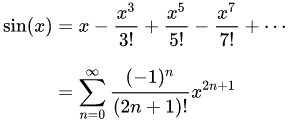
\includegraphics[width=\textwidth]{taylorpic.png}
\graphicspath{taylorpic.png}
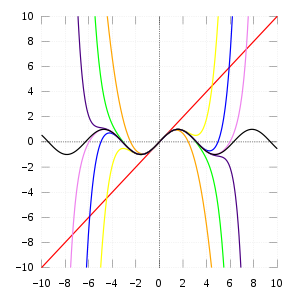
\includegraphics[width=\textwidth]{taaylor series.png}
\graphicspath{taylor series.png}
 \centering
 \caption{Taylor series of sine}

 
 \begin{minted}{python}
from math import*
import matplotlib
import matplotlib.pyplot as plt
import numpy as np

x=float(input("enter value of x="))

time = np.arange(0, 10, 0.1);
amplitude = np.sin(time)
plt.plot(time, amplitude)
plt.title('Sine wave')
plt.xlabel('Time')
plt.ylabel('Amplitude = sin(time)')
plt.grid(True, which='both')
plt.axhline(y=0, color='k')
plt.show()
plt.show()

for k in range(0,10,1):
    y=((-1)**k)*(x**(1+2*k))/factorial(1+2*k)
    print(y)
    print("sine taylor series is=")
    fig,ax = plt.subplots()
    plt.plot(y,'o-')
    ax.set(xlabel = 'time (s)',ylabel='amplitude',title = 'plotting of individual values of Taylor series in a sin Wave')
    ax.grid()
    plt.show()





    
\end{minted}
\begin{thebibliography}

\bibitem{lecture}
Question Paper
\end{thebibliography}

\end{document}
